\documentclass[12pt, a4paper]{article}

% PACKAGES
\usepackage{amsmath}         % For advanced math environments
\usepackage{geometry}        % For setting page margins
\usepackage{tikz}            % For drawing diagrams
\usepackage{amsfonts}        % For math fonts
\usepackage{amssymb}         % For math symbols
\usepackage{tabularx}        % For tables that fit page width

% HYPERREF SETUP (one call to the package with options)
\usepackage[colorlinks=true, linkcolor=blue, urlcolor=blue]{hyperref}

% PAGE GEOMETRY
\geometry{a4paper, margin=1in}

% DOCUMENT INFO
\title{Comprehensive Notes on Rotational Dynamics}
\author{}
\date{October 12, 2025}

\begin{document}

\maketitle
\tableofcontents
\newpage

\section{Moment of Inertia ($I$)}

The \textbf{moment of inertia} ($I$) is the rotational equivalent of mass, representing an object's resistance to angular acceleration. It depends on mass and how that mass is distributed around the axis of rotation.

\begin{itemize}
    \item \textbf{For a system of point masses:} \[I = \sum_{i} m_i r_i^2\]
    \item \textbf{For a continuous body:} \[I = \int r^2 dm\]
\end{itemize}

\subsection{Example: System of Point Masses}
Calculate the moment of inertia of the system below about an axis perpendicular to the page passing through the origin (0,0). Assume $m_1 = 2 \text{ kg}$ at $(3,0)$ and $m_2 = 4 \text{ kg}$ at $(0,2)$.

\begin{center}
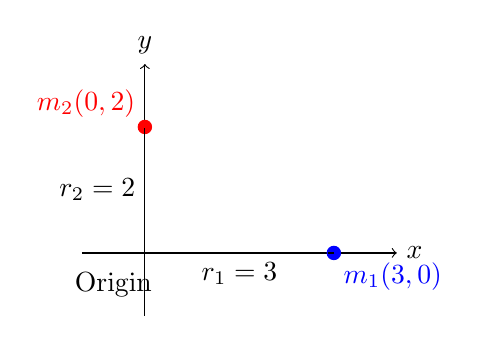
\begin{tikzpicture}[scale=0.8]
    \draw[->] (-1,0) -- (4,0) node[right] {$x$};
    \draw[->] (0,-1) -- (0,3) node[above] {$y$};
    \filldraw[blue] (3,0) circle (3pt) node[below right] {$m_1(3,0)$};
    \filldraw[red] (0,2) circle (3pt) node[above left] {$m_2(0,2)$};
    \draw[dashed] (0,0) -- (3,0) node[midway, below] {$r_1=3$};
    \draw[dashed] (0,0) -- (0,2) node[midway, left] {$r_2=2$};
    \node at (-0.5,-0.5) {Origin};
\end{tikzpicture}
\end{center}

\textbf{Solution:}
\[ I = \sum m_i r_i^2 = m_1 r_1^2 + m_2 r_2^2 \]
\[ I = (2 \text{ kg})(3 \text{ m})^2 + (4 \text{ kg})(2 \text{ m})^2 = 18 + 16 = 34 \text{ kg} \cdot \text{m}^2 \]

\subsection{Axis Theorems}

\subsubsection{Parallel Axis Theorem}
This theorem relates the moment of inertia about an axis through the center of mass ($I_{cm}$) to the moment of inertia about a parallel axis at a distance $d$.
\[ I = I_{cm} + Md^2 \]
Where $M$ is the total mass of the object.

\begin{center}
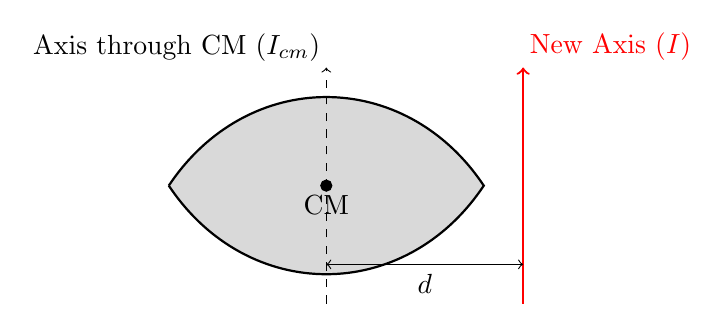
\begin{tikzpicture}[scale=1]
    % Draw a random shape
    \draw[fill=gray!30, thick] (0,0) .. controls (1,1.5) and (3,1.5) .. (4,0) .. controls (3,-1.5) and (1,-1.5) .. (0,0);
    % Center of mass
    \filldraw (2,0) circle (2pt) node[below] {CM};
    % Axis through CM
    \draw[->, dashed] (2,-1.5) -- (2,1.5) node[above left, inner sep=2pt] {Axis through CM ($I_{cm}$)};
    % Parallel axis
    \draw[->, thick, red] (4.5,-1.5) -- (4.5,1.5) node[above right, inner sep=2pt] {New Axis ($I$)};
    % Distance d
    \draw[<->] (2, -1) -- (4.5, -1) node[midway, below] {$d$};
\end{tikzpicture}
\end{center}

\textbf{Example:} Find the moment of inertia of a thin rod of mass $M$ and length $L$ about one of its ends. Given $I_{cm} = \frac{1}{12}ML^2$ and $d = L/2$.
\[ I_{end} = I_{cm} + M d^2 = \frac{1}{12}ML^2 + M \left(\frac{L}{2}\right)^2 = \frac{1}{12}ML^2 + \frac{1}{4}ML^2 = \frac{4}{12}ML^2 = \frac{1}{3}ML^2 \]

\subsubsection{Perpendicular Axis Theorem}
For any \textbf{planar object} (2D), the moment of inertia about an axis perpendicular to its plane ($I_z$) is the sum of the moments of inertia about two perpendicular axes in the plane ($I_x$ and $I_y$).
\[ I_z = I_x + I_y \]

\textbf{Example:} Find the moment of inertia of a uniform disk of mass $M$ and radius $R$ about a diameter. Given $I_z = \frac{1}{2}MR^2$ and by symmetry, $I_x = I_y$.
\[ I_z = I_x + I_y = 2I_x \implies I_{diameter} = I_x = \frac{I_z}{2} = \frac{1}{2} \left( \frac{1}{2}MR^2 \right) = \frac{1}{4}MR^2 \]

\section{Center of Mass (CM)}
For dynamics problems involving gravity, an extended object behaves as if its entire mass is concentrated at a single point, the \textbf{center of mass}. The change in gravitational potential energy of a rotating system depends on the vertical displacement of its center of mass.

For a system of point masses along a line (e.g., the y-axis):
\[ y_{CM} = \frac{\sum m_i y_i}{\sum m_i} = \frac{m_1 y_1 + m_2 y_2 + \dots}{m_1 + m_2 + \dots} \]
For a composite object, you can treat each component as a point mass located at its own center of mass.

\section{Rotational Kinetic Energy ($K_{rot}$)}
An object rotating with angular velocity $\omega$ has rotational kinetic energy.
\[ K_{rot} = \frac{1}{2} I \omega^2 \]
For an object that is both rotating and translating (rolling), the total kinetic energy is:
\[ K_{total} = K_{linear} + K_{rotational} = \frac{1}{2}mv^2 + \frac{1}{2}I\omega^2 \]

\section{Torque ($\tau$)}
\textbf{Torque} is the rotational equivalent of force, causing angular acceleration.
\[ \vec{\tau} = \vec{r} \times \vec{F} \quad \implies \quad \tau = rF\sin\theta \]
\textbf{Newton's Second Law for Rotation:} A net torque causes an angular acceleration $\alpha$.
\[ \sum \tau = I \alpha \]

\section{Angular Momentum ($L$) \& Conservation}
\textbf{Angular momentum} ($L$) is the rotational equivalent of linear momentum. For a rigid body:
\[ L = I \omega \]
\textbf{Conservation of Angular Momentum:} If the \textbf{net external torque} on a system is zero, its total angular momentum is conserved. This is key for analyzing collisions.
\[ \text{If } \sum \tau_{ext} = 0, \quad \text{then} \quad L_{initial} = L_{final} \implies I_i \omega_i = I_f \omega_f \]

\section{Summary Table: Linear vs. Rotational Motion}
\begin{center}
\begin{tabularx}{\textwidth}{| >{\hsize=0.9\hsize}X | >{\hsize=0.9\hsize}X | >{\hsize=1.2\hsize}X | >{\hsize=1.0\hsize}X |}
\hline
\textbf{Concept} & \textbf{Linear Motion} & \textbf{Rotational Motion} & \textbf{Relationship} \\
\hline
\textbf{Displacement} & Displacement ($x, s$) & Angular Displacement ($\theta$) & $s = r\theta$ \\
\hline
\textbf{Velocity} & Velocity ($v$) & Angular Velocity ($\omega$) & $v = r\omega$ \\
\hline
\textbf{Acceleration} & Acceleration ($a$) & Angular Acceleration ($\alpha$) & $a = r\alpha$ \\
\hline
\textbf{Inertia} & Mass ($m$) & Moment of Inertia ($I$) & $I = \int r^2 dm$ \\
\hline
\textbf{Kinetic Energy} & $K = \frac{1}{2}mv^2$ & $K = \frac{1}{2}I\omega^2$ & \\
\hline
\textbf{Cause of Accel.} & Force ($F$) & Torque ($\tau$) & $\tau = rF\sin\theta$ \\
\hline
\textbf{Newton's 2nd Law} & $\sum F = ma$ & $\sum \tau = I\alpha$ & \\
\hline
\textbf{Momentum} & Momentum ($p=mv$) & Angular Momentum ($L=I\omega$) & \\
\hline
\textbf{Conservation Law} & If $\sum F_{ext}=0$, $p$ is conserved. & If $\sum \tau_{ext}=0$, $L$ is conserved. & \\
\hline
\end{tabularx}
\end{center}

\newpage
\section{Application Problems with Solutions}

\subsection{Problem 1: Satellite Solar Panels (SPhO 2024)}
\textbf{Problem:} A satellite with its solar panels folded has a moment of inertia of $110 \text{ kg m}^2$ and is spun to rotate at $5.2 \text{ rad s}^{-1}$. After it is released, its solar panels are extended, and the new moment of inertia is $230 \text{ kg m}^2$. Calculate the decrease in rotational kinetic energy.

\textbf{Explanation:} When the panels are extended, no external torque acts on the satellite. Therefore, its angular momentum is conserved. We use this to find the final angular velocity. Then, we can calculate the initial and final kinetic energies to find the decrease.

\textbf{Solution:}
\begin{enumerate}
    \item \textbf{Find the final angular velocity using conservation of angular momentum:}
    \[ L_i = L_f \implies I_i \omega_i = I_f \omega_f \]
    \[ (110 \text{ kg m}^2)(5.2 \text{ rad s}^{-1}) = (230 \text{ kg m}^2) \omega_f \]
    \[ \omega_f = \frac{110 \times 5.2}{230} = 2.487 \text{ rad s}^{-1} \]

    \item \textbf{Calculate the initial and final kinetic energies:}
    \[ K_i = \frac{1}{2} I_i \omega_i^2 = \frac{1}{2} (110)(5.2)^2 = 1487.2 \text{ J} \]
    \[ K_f = \frac{1}{2} I_f \omega_f^2 = \frac{1}{2} (230)(2.487)^2 = 712.2 \text{ J} \]

    \item \textbf{Find the decrease in kinetic energy:}
    \[ \Delta K = K_i - K_f = 1487.2 \text{ J} - 712.2 \text{ J} = 775 \text{ J} \]
    The work done to extend the panels accounts for this energy loss.
\end{enumerate}

\subsection{Problem 2: Compound Pendulum Collision (SPhO 2022)}
\textbf{Problem:} A pendulum consists of a uniform rod ($L=50$ cm, $M_r=1.5$ kg) and a thin disc ($D=15$ cm, $M_d=3.0$ kg) attached to its end B. It pivots at A. A small object ($m=0.1$ kg) with horizontal speed $v=30 \text{ m s}^{-1}$ strikes and sticks to the system at B. Find the greatest angle the rod makes with the downward vertical.

\textbf{Explanation:} This is a three-part problem. First, calculate the total moment of inertia of the pendulum. Second, use conservation of angular momentum for the collision to find the angular velocity just after impact. Third, use conservation of mechanical energy for the subsequent swing to find the maximum angle.

\textbf{Solution:}
\begin{enumerate}
    \item \textbf{Calculate the system's moment of inertia about the pivot A:}
    \begin{itemize}
        \item Rod (pivot at end): $I_{rod} = \frac{1}{3}M_r L^2 = \frac{1}{3}(1.5)(0.5)^2 = 0.125 \text{ kg m}^2$.
        \item Disc (use Parallel Axis Theorem): The pivot is at distance $d=L=0.5$ m from the disc's center. Radius $R = D/2 = 0.075$ m.
        \[ I_{disc} = I_{cm} + M_d d^2 = \frac{1}{2}M_d R^2 + M_d L^2 \]
        \[ I_{disc} = \frac{1}{2}(3.0)(0.075)^2 + (3.0)(0.5)^2 = 0.0084 + 0.75 = 0.7584 \text{ kg m}^2 \]
        \item Object (after sticking): $I_{obj} = m L^2 = (0.1)(0.5)^2 = 0.025 \text{ kg m}^2$.
        \item Total moment of inertia of the final system:
        \[ I_{sys} = I_{rod} + I_{disc} + I_{obj} = 0.125 + 0.7584 + 0.025 = 0.9084 \text{ kg m}^2 \]
    \end{itemize}
    \item \textbf{Apply conservation of angular momentum for the collision:}
    \[ L_i = L_f \implies L_{obj, before} = L_{sys, after} \]
    \[ (L)(m v) = I_{sys} \omega_f \]
    \[ (0.5)(0.1)(30) = (0.9084) \omega_f \implies \omega_f = \frac{1.5}{0.9084} = 1.651 \text{ rad s}^{-1} \]
    \item \textbf{Apply conservation of energy for the swing:} The initial rotational KE is converted to gravitational PE.
    \[ K_i = U_f \implies \frac{1}{2} I_{sys} \omega_f^2 = (M_{total}) g \Delta h_{CM} \]
    First, find the center of mass ($y_{CM}$) of the final system, measured from pivot A.
    \[ y_{CM} = \frac{M_r(L/2) + M_d(L) + m(L)}{M_r + M_d + m} = \frac{1.5(0.25) + 3.0(0.5) + 0.1(0.5)}{1.5+3.0+0.1} = \frac{1.925}{4.6} = 0.4185 \text{ m} \]
    The change in height of the CM is $\Delta h_{CM} = y_{CM}(1-\cos\theta)$.
    \[ \frac{1}{2} (0.9084) (1.651)^2 = (4.6)(9.81)(0.4185)(1-\cos\theta) \]
    \[ 1.239 = 18.89(1-\cos\theta) \]
    \[ 1-\cos\theta = \frac{1.239}{18.89} = 0.0656 \implies \cos\theta = 0.9344 \]
    \[ \theta = \arccos(0.9344) = 20.9^\circ \]
\end{enumerate}

\subsection{Problem 3: Composite Rod Swing (SPhO 2020)}
\textbf{Problem:} A rod ($L=1.0$ m, $r=1.0$ cm) consists of a zinc section ($L_z=0.5$ m) and a copper section ($L_c=0.5$ m). The zinc end is pivoted at O. The rod is released from a horizontal position. Find its angular velocity when it is vertical. (Densities: $\rho_z=7135$, $\rho_c=8940$ kg m$^{-3}$).

\textbf{Explanation:} This problem uses the conservation of mechanical energy. The loss in gravitational potential energy of the rod's center of mass is converted into rotational kinetic energy. We must first find the masses, the center of mass, and the total moment of inertia of the composite rod.

\textbf{Solution:}
\begin{enumerate}
    \item \textbf{Calculate masses of the sections:} Volume $V = \pi r^2 L_{sec} = \pi (0.01)^2 (0.5) = 1.571 \times 10^{-4} \text{ m}^3$.
    \[ M_z = \rho_z V = (7135)(1.571 \times 10^{-4}) = 1.121 \text{ kg} \]
    \[ M_c = \rho_c V = (8940)(1.571 \times 10^{-4}) = 1.404 \text{ kg} \]
    Total Mass $M_{tot} = 1.121 + 1.404 = 2.525 \text{ kg}$.
    \item \textbf{Calculate total moment of inertia about pivot O:}
    \begin{itemize}
        \item Zinc section (pivoted at its end): $I_z = \frac{1}{3}M_z L_z^2 = \frac{1}{3}(1.121)(0.5)^2 = 0.0934 \text{ kg m}^2$.
        \item Copper section (use Parallel Axis Theorem): Its CM is at distance $d = L_z + L_c/2 = 0.5+0.25 = 0.75$ m from O.
        \[ I_c = I_{cm} + M_c d^2 = \frac{1}{12}M_c L_c^2 + M_c d^2 \]
        \[ I_c = \frac{1}{12}(1.404)(0.5)^2 + (1.404)(0.75)^2 = 0.0292 + 0.7898 = 0.8190 \text{ kg m}^2 \]
        \item Total moment of inertia: $I_{tot} = I_z + I_c = 0.0934 + 0.8190 = 0.9124 \text{ kg m}^2$.
    \end{itemize}
    \item \textbf{Apply conservation of energy:} Loss in PE = Gain in Rotational KE.
    \[ M_{tot} g h_{CM} = \frac{1}{2}I_{tot}\omega^2 \]
    First, find the initial height (distance from pivot) of the composite CM. The rod is horizontal, so we find its position along the rod from O.
    \[ x_{CM} = \frac{M_z(L_z/2) + M_c(L_z+L_c/2)}{M_z+M_c} = \frac{1.121(0.25) + 1.404(0.75)}{2.525} = \frac{0.280 + 1.053}{2.525} = 0.528 \text{ m} \]
    When the rod swings from horizontal to vertical, the CM drops by this distance, so $h_{CM} = x_{CM} = 0.528$ m.
    \[ (2.525)(9.81)(0.528) = \frac{1}{2}(0.9124)\omega^2 \]
    \[ 13.08 = 0.4562 \omega^2 \implies \omega^2 = \frac{13.08}{0.4562} = 28.67 \]
    \[ \omega = \sqrt{28.67} = 5.35 \text{ rad s}^{-1} \]
\end{enumerate}

\subsection{Problem 4: Block and Rod Collision (SPhO 2021)}
\textbf{Problem:} A 50 g block slides from rest down a frictionless surface from a height $h=20$ cm and sticks to the end of a uniform rod (100 g, 40 cm). The rod pivots about point O at its top. Find the angle $\theta$ the rod swings through before stopping.

\textbf{Explanation:} This is another multi-step problem. First, find the block's speed at the bottom using energy conservation. Second, use angular momentum conservation for the collision. Third, use energy conservation again for the swing to find the angle.

\textbf{Solution:}
\begin{enumerate}
    \item \textbf{Find the block's speed before impact:}
    \[ m_b g h = \frac{1}{2} m_b v^2 \implies v = \sqrt{2gh} = \sqrt{2(9.81)(0.20)} = 1.981 \text{ m s}^{-1} \]
    \item \textbf{Apply conservation of angular momentum for the collision:}
    The initial angular momentum is from the block. The final system is the rod + block.
    \[ L_i = (L)(m_b v) = (0.4)(0.05)(1.981) = 0.03962 \text{ kg m}^2\text{s}^{-1} \]
    The final moment of inertia of the system about pivot O is:
    \[ I_{sys} = I_{rod} + I_{block} = \frac{1}{3}M_r L^2 + m_b L^2 = (\frac{1}{3}M_r + m_b)L^2 \]
    \[ I_{sys} = (\frac{1}{3}(0.10) + 0.05)(0.4)^2 = (0.08333)(0.16) = 0.01333 \text{ kg m}^2 \]
    Now find the angular velocity $\omega$ just after collision:
    \[ L_i = I_{sys} \omega \implies 0.03962 = 0.01333 \omega \implies \omega = 2.972 \text{ rad s}^{-1} \]
    \item \textbf{Apply conservation of energy for the swing:}
    The initial rotational KE is converted to gravitational PE.
    \[ K_i = U_f \implies \frac{1}{2} I_{sys} \omega^2 = \Delta U_{rod} + \Delta U_{block} \]
    \[ \Delta U_{rod} = M_r g \Delta h_{rod} = M_r g \frac{L}{2}(1-\cos\theta) \]
    \[ \Delta U_{block} = m_b g \Delta h_{block} = m_b g L(1-\cos\theta) \]
    \[ \frac{1}{2} (0.01333)(2.972)^2 = \left( M_r g \frac{L}{2} + m_b g L \right)(1-\cos\theta) \]
    \[ 0.05889 = \left( (0.1)(9.81)(0.2) + (0.05)(9.81)(0.4) \right)(1-\cos\theta) \]
    \[ 0.05889 = (0.1962 + 0.1962)(1-\cos\theta) = 0.3924(1-\cos\theta) \]
    \[ 1-\cos\theta = \frac{0.05889}{0.3924} = 0.150 \implies \cos\theta = 0.850 \]
    \[ \theta = \arccos(0.850) = 31.8^\circ \]
\end{enumerate}

\end{document}